
The first signals sent by Cortex M3 are transmitted to the uartlite element. The main scope of our studies on this component aims at understanding which the meaning of the bits sent from tx channel is and how the processor can control them. In order to reach our purpose, we studied the handshake protocol between these two elements of the design and we analysed the tx’s output with the help of the documentation.


{\color{Blue}\subsection{Uart Decoding}}
%explain manual decoding of uart's tx

The communication between Cortex M3 and uartlite is achieved using a set of reads and writes on the same three addresses: \verb+0x4010_0004+, \verb+0x4010_000c+ (write only) and \verb+0x4010_0008+ (read only).
While the first 16 bits are the base address for the communication with uartlite (how it is possible to see in the address editor of the block design), the last 16 define the offset specified in the uartlite's product guide \cite[Chapter2.Register Space]{AXIUartguide}. In particular, the offset \verb+0x0004+ is used as FIFO queue for the data which should be transmitted on tx channel.
\newline

Unfortunately, to know the value of the words sent wasn’t enough to understand the decoding procedure used on transmitter channel. We found also:
{\flushleft
\begin{description}

\item[Baud Rate:] After hypothesising a Baud Rate which was about 115740 bit/sec (in according to the sampling period used 8.34 us for the tx channel in \textit{tb m3 for arty}), we discovered the more precise value of \textbf{175200 bit/sec} in the \textit{IP configuration} of uartlite (the nearest value to 115740 bit/sec among the possible choices), like showed in Figure \ref{ip_config}.
\item[Data length:] Defined in the \textit{IP configuration}
of the uartlite, the data length is \textbf{8 bits} without parity check, like showed in Figure \ref{ip_config}.

\item[Start and End Bits:] Reading the documentation about the UART communication protocol\cite{UartBasics} we discovered the presence of a \textbf{start bit 0} and an \textbf{end bit 1} used to enclose the 8 bits word.

\item[Data Order:] Analysing the sequence of bits on tx channel and the values written on address \verb+0x4010_0004+,  we found the character \verb+0x0d+ (carriage return in ASCII code) which is written \textbf{starting from the last significant bit} (unfortunately, the previous characters \verb+0x2a+ are too symmetric, thus we chose \verb+0x0d+). In the Figure \ref{0x0d_waveform} it is possible to see the piece of waveform analised.
\end{description}
}

At the end, we can conclude that the transmission on tx channel is defined with a sequence of 8 bits words enclosed by the starting bit 0 and the ending bit 1 and taken from the address \verb+0x4010_0004+ starting by the last significant bit.

\begin{figure}[!hb]
  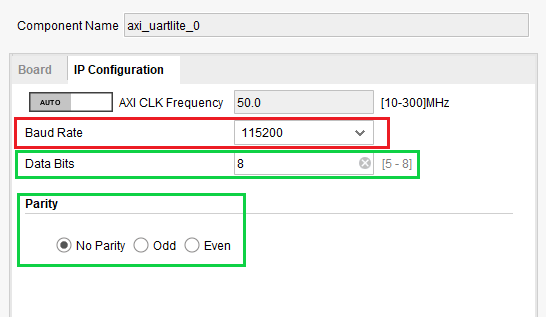
\includegraphics{./../../img/Images/uartlite_ip_configuration_col}
  \caption{IP configuration with {\color{Red}Baud Rate} and {\color{Green} bits} definition}
  \label{ip_config}
\end{figure}

\begin{figure}[!hb]
  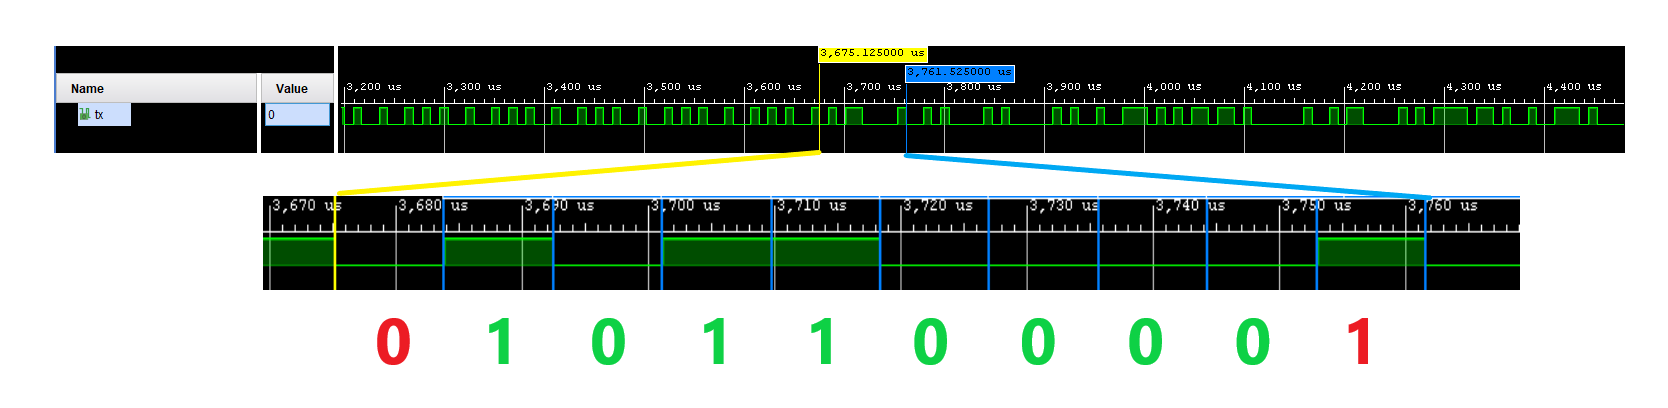
\includegraphics[width=\textwidth]{./../../img/Images/uart_tx_0x0d}
  \caption{%\verb+0x0d+ ({\color{Green}\verb+1101_0000+} in binary) in the tx channel waveform with {\color{Red}start} and {\color{Red}end} bits ---> gives error for extra } but it is strange
  %: todo try to add a caption
  }
  \label{0x0d_waveform}
\end{figure}


{\color{Blue}\subsection{Decoding Software}}
%explain cose used for deconding
After analysing the signals transmitted by the uartlite and after understanding their encoding, we wrote in the file Verilog of the testbench some line of code in order to make automatic the decoding of the output and, at the same time, write it on a text file. The main operation of this code is executed by the always block showed by the following Figure \ref{always_block}.

\begin{figure}[!hbp]
  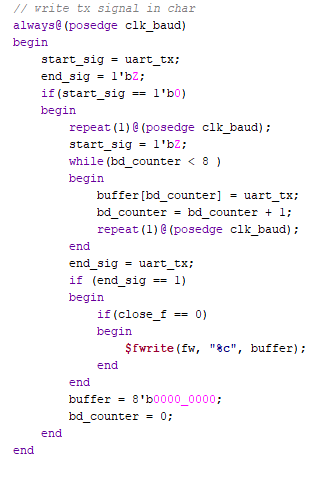
\includegraphics{./../../img/Images/tx_decoding_block} %todo: try to center, possible delete
  \caption{The always block.}
  \label{always_block}
\end{figure}

It waits until the first 0 on output tx, then it writes the first eight bits and, at the end, it takes the nineth bit as ending bit and it waits the first 0 value to execute the block again.
All the bits are saved in three register variables ({\verb+start_sig+}, {\verb+buffer+} and { \verb+end_sig+}, respectively) and cleaned a clock’s cycle after being writtten or, for the { \verb+end_sig+}, at the beginning of the always block using value Z for one bit variable and 0 for the buffer.
It is important to explain that the writing on the text file is only for the buffer and it happens one clock’s cycle after that all the buffer’s bits are defined checking the { \verb+end_sig+}’s value (1 for correct transmission) and only if the file is opening (the file is opened at the beginning of initial block and its closing is managed by another always block).
Moreover, the assigning and the checking of the tx’s values occur at the positive edge of the { \verb+clk_baud+}. This is because we noticed that the bit changing is quite aligned with that clock, in fact, during the communication the output tx changes the bit 1.170 us before the positive edge of the { \verb+clk_baud+}.
